\subsection{Qualitative variables}
\label{sec:eda-cualitativas}

The categorical variables are reported in two blocks by unit of analysis:
\texttt{periodo} (period of the day) and \texttt{llovio} exist only at
hourly resolution; the exceedance indicators derive from the MDA8 and exist
only at daily resolution. Mixing them would replicate each daily value 24
times. The bases are $n = 640{,}583$ station-hour records and
$n = 26{,}691$ station-days.

\subsubsection{Frequency distribution}

\Cref{tab:freq-horaria} gathers the hourly variables. With 2025 complete, the
four seasons are balanced (24.79\,\% to 25.16\,\%), so no seasonal contrast is
an artifact of the observation window. \texttt{periodo} is uniform by
construction: four 6-hour blocks over a complete hourly grid.
\texttt{llovio} is the only hourly variable with missing data (19,360
records, 3.02\,\%), which are kept as a separate category rather than
assigned to ``did not rain''; it rains in 1.49\,\% of the hours with a
measurement. \texttt{tipo\_dia} replaces the weekend dummy because it
separates Saturday from Sunday, whose traffic patterns differ, and isolates
the 81 public holidays of the period.

\begin{table}[t]
  \centering
  \caption{Absolute and relative frequency of the qualitative variables at
    station-hour resolution ($n = 640{,}583$). Percentages are over records
    with valid data.}
  \label{tab:freq-horaria}
  \small
  \begin{tabular}{llrr}
    \toprule
    Variable & Level & Frequency & \% \\
    \midrule
    \multirow{4}{*}{\texttt{temporada}}
                                  & Winter    &   158,783 &  24.79 \\
                                  & Spring    &   161,184 &  25.16 \\
                                  & Summer    &   161,184 &  25.16 \\
                                  & Autumn    &   159,432 &  24.89 \\
    \midrule
    \multirow{4}{*}{\texttt{periodo}}
                                  & Early morning &   160,145 &  25.00 \\
                                  & Morning   &   160,146 &  25.00 \\
                                  & Afternoon &   160,146 &  25.00 \\
                                  & Night     &   160,146 &  25.00 \\
    \midrule
    \multirow{4}{*}{\texttt{tipo\_dia}}
                                  & Weekday   &   434,879 &  67.89 \\
                                  & Saturday  &    88,392 &  13.80 \\
                                  & Sunday    &    88,728 &  13.85 \\
                                  & Holiday   &    28,584 &   4.46 \\
    \midrule
    \multirow{3}{*}{\texttt{llovio}}
                                  & No (0)    &   611,952 &  98.51 \\
                                  & Yes (1)   &     9,271 &   1.49 \\
                                  & Missing   &    19,360 &    --- \\
    \bottomrule
  \end{tabular}
\end{table}

\Cref{tab:freq-diaria} presents the daily block. The three MDA8 indicators
share the same 1,591 missing records (5.96\,\%), the station-days whose MDA8
did not reach the completeness of 18 of 24 windows; \texttt{excede\_1h} does
not share them because it is computed on the hourly maximum.

\begin{table}[t]
  \centering
  \caption{Absolute and relative frequency of the exceedance indicators at
    station-day resolution ($n = 26{,}691$; valid $= 25{,}100$ for the MDA8
    indicators).}
  \label{tab:freq-diaria}
  \small
  \begin{tabular}{llrr}
    \toprule
    Variable & Level & Frequency & \% \\
    \midrule
    \multirow{3}{*}{\texttt{excede\_anio\_1} (65 ppb)}
                                        & No        &  22,275 &  88.75 \\
                                        & Yes       &   2,825 &  11.25 \\
                                        & Missing       &   1,591 &    --- \\
    \midrule
    \multirow{3}{*}{\texttt{excede\_anio\_3} (60 ppb)}
                                        & No        &  20,864 &  83.12 \\
                                        & Yes       &   4,236 &  16.88 \\
                                        & Missing       &   1,591 &    --- \\
    \midrule
    \multirow{3}{*}{\texttt{excede\_anio\_5} (51 ppb)}
                                        & No        &  17,079 &  68.04 \\
                                        & Yes       &   8,021 &  31.96 \\
                                        & Missing       &   1,591 &    --- \\
    \midrule
    \multirow{2}{*}{\texttt{excede\_1h} (90 ppb)}
                                        & No        &  24,497 &  91.78 \\
                                        & Yes       &   2,194 &   8.22 \\
    \bottomrule
  \end{tabular}
\end{table}

\subsubsection{The monitoring station}

Fourteen of the 15 stations record 43,824 observations each, the complete
hourly grid from 2021-01-01 to 2025-12-31; \texttt{NO3} records 27,047
because it started operating on 1 December 2022. The difference is one of
coverage, not quality: within its window, \texttt{NO3} also has a complete
grid, and its share of hours with measured \ce{O3} is within the range of the
rest of the network. \texttt{periodo}, the only ordinal variable, has median
\texttt{tarde} (afternoon) over the 611,601 hours with measured \ce{O3},
because missing data concentrate at night.

\subsubsection{Class balance}

\Cref{fig:eda-cual-excedencias} shows the balance of the three MDA8
indicators. At the current 65 ppb threshold, exceedances are 11.25\,\% of
valid station-days: a classifier that always predicts the majority class
reaches 88.75\,\% accuracy without capturing the phenomenon, so accuracy is
discarded as a metric in favor of sensitivity, specificity and area under
the ROC curve. The 51 ppb threshold, with 31.96\,\%, offers a substantially
better balance and is the main modeling scenario.

\begin{figure}[t]
  \centering
  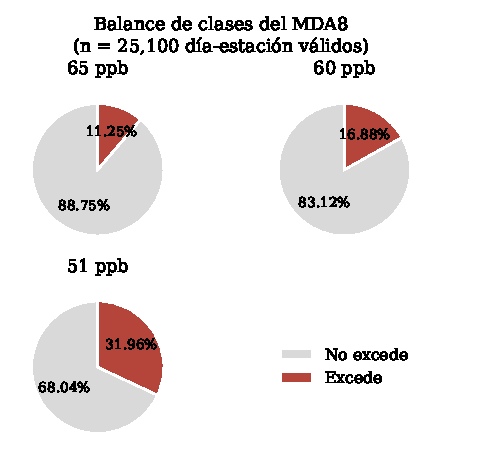
\includegraphics[width=\linewidth]{eda_cual_excedencias.pdf}
  \caption{Class balance of the MDA8 exceedance indicators for the three
    gradual compliance thresholds of NOM-020-SSA1-2021
    (\cref{tab:nom-limites}).}
  \label{fig:eda-cual-excedencias}
\end{figure}
